\documentclass[tikz,border=12pt]{standalone}
\usepackage[T1]{fontenc}
\usepackage{mathptmx}
\usepackage{tikz}
\usetikzlibrary{arrows.meta,positioning,shapes.geometric,fit,calc,backgrounds}

\definecolor{boxfill}{HTML}{EEECFE}
\definecolor{boxdraw}{HTML}{5B4B8A}
\definecolor{clusterfill}{HTML}{FFF8DC}
\definecolor{clusterdraw}{HTML}{B59F20}
\definecolor{hostfill}{HTML}{FBF9EE}
\definecolor{hostdraw}{HTML}{6E6615}
\definecolor{extfill}{HTML}{FCFCF7}
\definecolor{extdraw}{HTML}{6E6615}

\begin{document}
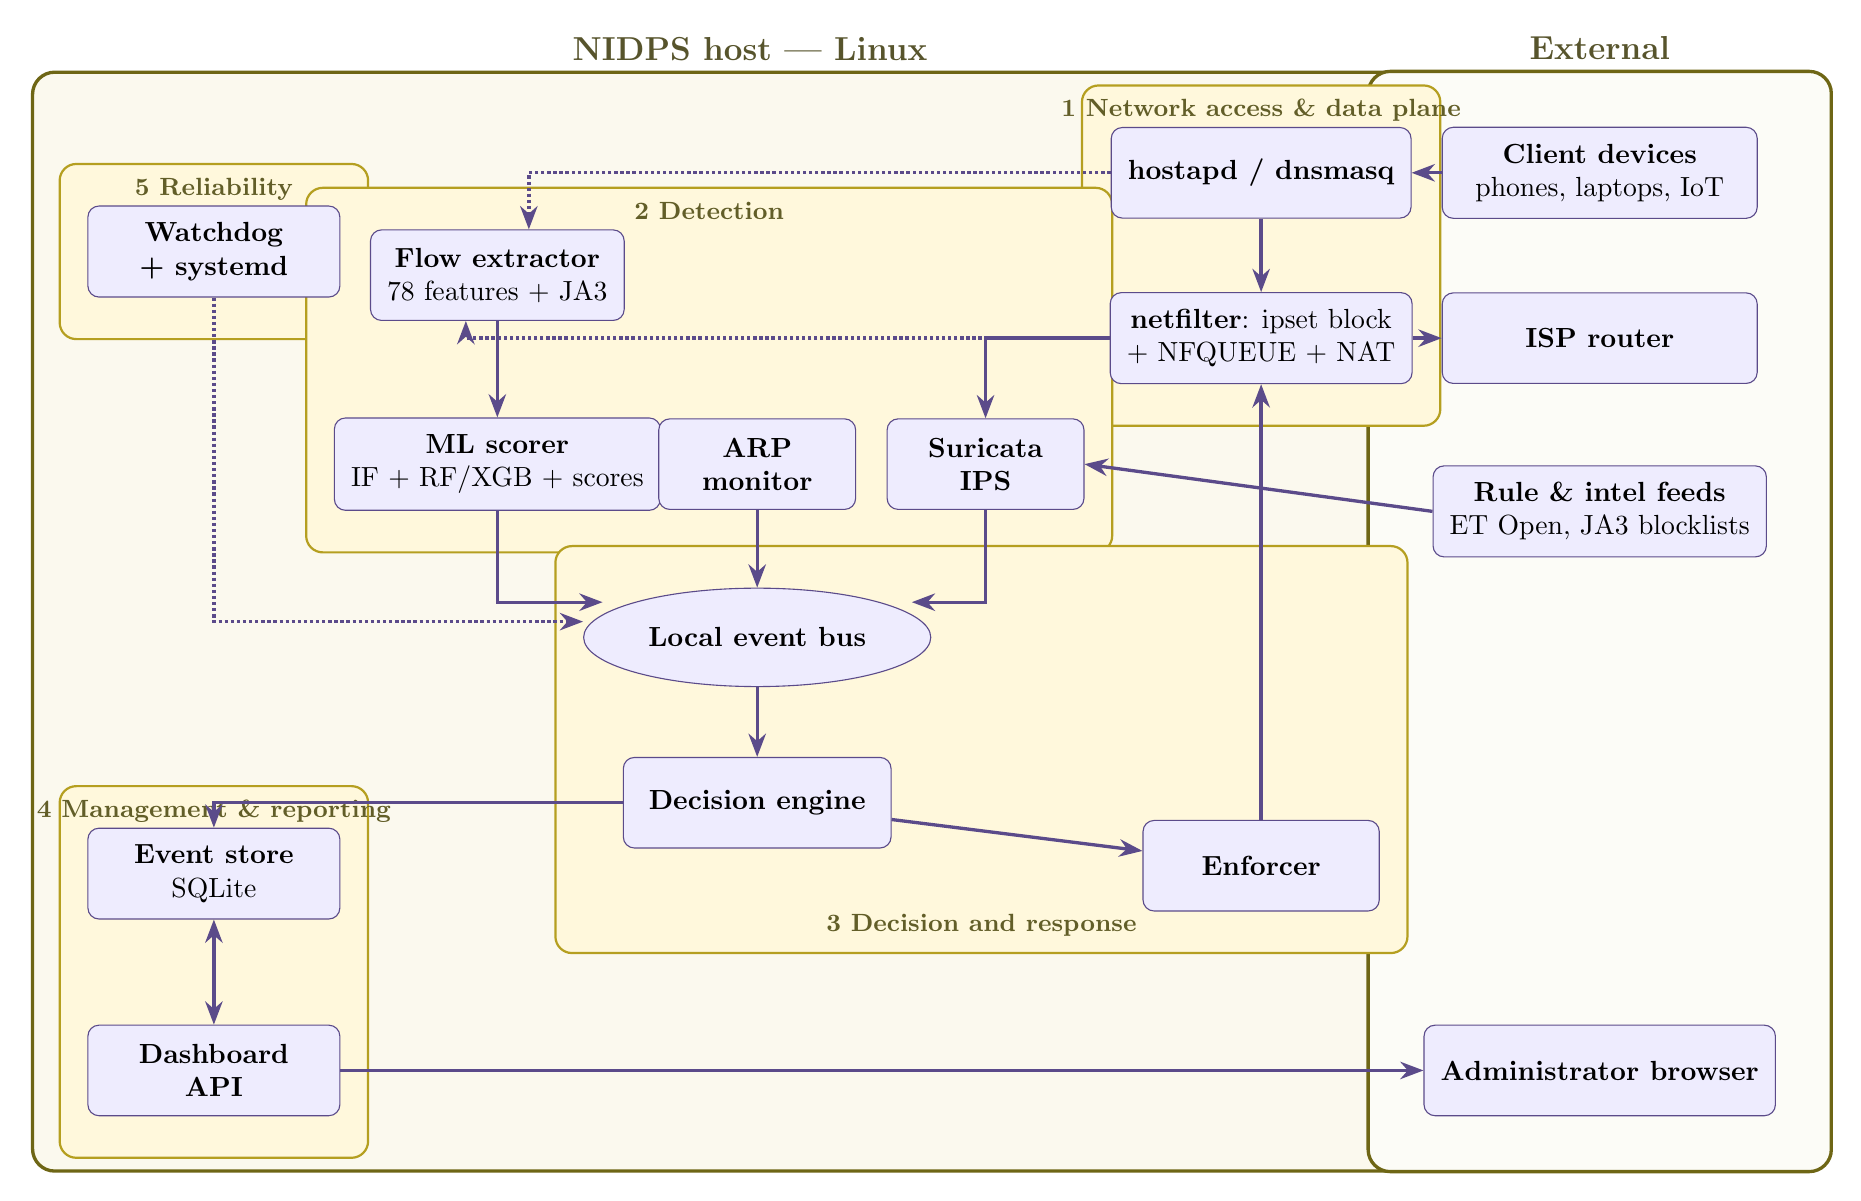
\begin{tikzpicture}[
  font=\normalsize,
  >=Stealth,
  component/.style={draw=boxdraw, fill=boxfill, rounded corners=4pt,
    align=center, inner sep=6pt, minimum height=1.15cm, minimum width=2.6cm, font=\normalsize},
  compbold/.style={draw=boxdraw, fill=boxfill, rounded corners=4pt,
    align=center, inner sep=6pt, minimum height=1.15cm, minimum width=2.6cm, font=\normalsize\bfseries},
  bus/.style={draw=boxdraw, fill=boxfill, ellipse, align=center,
    inner sep=5pt, minimum width=3.8cm, minimum height=1.25cm, font=\normalsize\bfseries},
  arr/.style={->, very thick, draw=boxdraw},
  biarr/.style={<->, very thick, draw=boxdraw},
  sarr/.style={->, very thick, densely dotted, draw=boxdraw}
]

% ----------------- EXTERNAL COLUMN (Right) -----------------
\node[component, minimum width=4.0cm] (clients) at (19.4, 6.8) {\textbf{Client devices}\\phones, laptops, IoT};
\node[component, minimum width=4.0cm] (isp)     at (19.4, 4.7) {\textbf{ISP router}};
\node[component, minimum width=4.0cm] (feeds)   at (19.4, 2.5) {\textbf{Rule \& intel feeds}\\ET Open, JA3 blocklists};
\node[component, minimum width=4.0cm] (admin)   at (19.4, -4.6) {\textbf{Administrator browser}};

% ----------------- NIDPS HOST (Left) -----------------
\begin{scope}[local bounding box=hostbox]

  % Lane 1: Reliability (top) & Management (bottom)
  \node[compbold, minimum width=3.2cm] (wd) at (1.8, 5.8) {Watchdog\\+ systemd};
  \node[component, minimum width=3.2cm] (store) at (1.8, -2.1) {\textbf{Event store}\\SQLite};
  \node[compbold, minimum width=3.2cm] (dash) at (1.8, -4.6) {Dashboard\\API};

  % Lane 2: Flow extractor & ML Scorer
  \node[component, minimum width=3.2cm] (flow) at (5.4, 5.5) {\textbf{Flow extractor}\\78 features + JA3};
  \node[component, minimum width=3.2cm] (ml) at (5.4, 3.1) {\textbf{ML scorer}\\IF + RF/XGB + scores};

  % Lane 3: ARP Monitor, Event bus, Decision engine
  \node[compbold, minimum width=2.5cm] (arp) at (8.7, 3.1) {ARP\\monitor};
  \node[bus] (bus) at (8.7, 0.9) {Local event bus};
  \node[compbold, minimum width=3.4cm] (dec) at (8.7, -1.2) {Decision engine};

  % Lane 4: Suricata IPS
  \node[compbold, minimum width=2.5cm] (suri) at (11.6, 3.1) {Suricata\\IPS};

  % Lane 5: Data plane (top) & Enforcer (bottom)
  \node[compbold, minimum width=3.4cm] (hapd) at (15.1, 6.8) {hostapd / dnsmasq};
  \node[component, minimum width=3.4cm] (nf) at (15.1, 4.7) {\textbf{netfilter}: ipset block\\+ NFQUEUE + NAT};
  \node[compbold, minimum width=3.0cm] (enf) at (15.1, -2.0) {Enforcer};

\end{scope}

% ----------------- BACKGROUND CLUSTERS -----------------
\begin{scope}[on background layer]
  % 1. Outer host box first
  \node[draw=hostdraw, fill=hostfill, very thick, rounded corners=8pt, inner sep=20pt,
        fit=(hostbox), label={[font=\large\bfseries, text=olive!50!black]above:NIDPS host --- Linux}] (host) {};

  % 2. Outer external box
  \node[draw=extdraw, fill=extfill, very thick, rounded corners=8pt, inner sep=20pt,
        fit=(clients)(feeds)(isp)(admin), label={[font=\large\bfseries, text=olive!50!black]above:External}] (ext) {};

  % 3. Inner subsystem clusters drawn on top of hostfill
  \node[draw=clusterdraw, fill=clusterfill, thick, rounded corners=6pt, inner ysep=15pt, inner xsep=10pt,
        fit=(wd)] (c5) {};
  \node[font=\small\bfseries, text=olive!60!black, anchor=north] at ([yshift=-2pt]c5.north) {5 Reliability};

  \node[draw=clusterdraw, fill=clusterfill, thick, rounded corners=6pt, inner ysep=15pt, inner xsep=10pt,
        fit=(hapd)(nf)] (c1) {};
  \node[font=\small\bfseries, text=olive!60!black, anchor=north] at ([yshift=-2pt]c1.north) {1 Network access \& data plane};

  \node[draw=clusterdraw, fill=clusterfill, thick, rounded corners=6pt, inner ysep=15pt, inner xsep=10pt,
        fit=(flow)(ml)(arp)(suri)] (c2) {};
  \node[font=\small\bfseries, text=olive!60!black, anchor=north] at ([yshift=-2pt]c2.north) {2 Detection};

  \node[draw=clusterdraw, fill=clusterfill, thick, rounded corners=6pt, inner ysep=15pt, inner xsep=10pt,
        fit=(bus)(dec)(enf)] (c3) {};
  \node[font=\small\bfseries, text=olive!60!black, anchor=south] at ([yshift=3pt]c3.south) {3 Decision and response};

  \node[draw=clusterdraw, fill=clusterfill, thick, rounded corners=6pt, inner ysep=15pt, inner xsep=10pt,
        fit=(store)(dash)] (c4) {};
  \node[font=\small\bfseries, text=olive!60!black, anchor=north] at ([yshift=-2pt]c4.north) {4 Management \& reporting};
\end{scope}

% ----------------- DATA FLOW CONNECTIONS -----------------
% External traffic flow
\draw[arr] (clients) -- (hapd);
\draw[arr] (hapd) -- (nf);
\draw[arr] (nf) -- (isp);

% Passive copy to flow extractor
\draw[sarr] (hapd.west) -| ([xshift=4mm]flow.north);
\draw[sarr] (nf.west) -| ([xshift=-4mm]flow.south);

% Detection pipeline
\draw[arr] (flow) -- (ml);
\draw[arr] (feeds.west) -- (suri.east);
\draw[arr] (nf.west) -| (suri.north);

% Feeds into Local Event Bus
\draw[arr] (ml.south) |- ([xshift=-4mm]bus.north west);
\draw[arr] (arp.south) -- (bus.north);
\draw[arr] (suri.south) |- ([xshift=4mm]bus.north east);

% Watchdog status into Event Bus (routed cleanly around the left)
\draw[sarr] (wd.south) |- ([yshift=2mm]bus.west);

% Decision & Enforcement
\draw[arr] (bus) -- (dec);
\draw[arr] (dec) -- (enf);

% Enforcer updates netfilter block rule (straight vertical up)
\draw[arr] (enf.north) -- (nf.south);

% Management & Storage
\draw[arr] (dec.west) -| (store.north);
\draw[biarr] (store) -- (dash);

% Admin UI across the bottom
\draw[arr] (dash.east) -- (admin.west);

\end{tikzpicture}
\end{document}
